% 第9章第3节：积分泛函的变分（一阶变分的计算、Euler--Lagrange方程、边界条件）。

\section{积分泛函的变分}
\label{sec:opt-fn-integral}

最常见的目标泛函是对局部代价的积分：每个位置$x$上，代价由$x$、函数值$u(x)$和导数$u'(x)$决定，再沿整个区间累加。本节固定这类目标，先计算它的一阶变化，再分别用内部扰动和边界扰动从最优条件中提取两类信息：区间内部的微分方程与边界上的条件。

\subsection{一阶变分的计算}
\label{sec:opt-fn-first-variation}

\paragraph{一维积分泛函}
设$F(x,s,p)$是定义在$[a,b]\times\mathbb R\times\mathbb R$上的函数，称为密度，目标为
\begin{equation}
 J(u)=\int_a^bF\bigl(x,u(x),u'(x)\bigr)\,dx .
 \label{eq:opt-fn-integral-functional}
\end{equation}
用$F_s$、$F_p$表示$F$对第二、第三个变量的偏导数；沿候选$u$求值时，习惯上写成$F_u=F_s(x,u,u')$、$F_{u'}=F_p(x,u,u')$。记号$F_{u'}$表示“对导数所在的那个变量求偏导”，不是对$u'$这个函数求导。

\begin{theorem}[积分泛函的方向导数]
\label{thm:opt-fn-first-variation}
设$F$对$(s,p)$连续可微，$u,h$使$J(u+th)$对$|t|\le t_0$有限，并存在可积函数$m$，使对几乎所有$x$及所有$|\tau|\le t_0$，
\begin{equation}
 \bigl|F_s(x,u+\tau h,u'+\tau h')\,h+F_p(x,u+\tau h,u'+\tau h')\,h'\bigr|\le m(x) .
 \label{eq:opt-fn-domination}
\end{equation}
则
\begin{equation}
 J'(u;h)=\int_a^b\bigl(F_u\,h+F_{u'}\,h'\bigr)\,dx .
 \label{eq:opt-fn-first-variation}
\end{equation}
\end{theorem}

\begin{proof}
固定$x$，$\tau\mapsto F(x,u+\tau h,u'+\tau h')$连续可微，由中值定理，对$0<|t|\le t_0$，差商$\bigl(F(x,u+th,u'+th')-F(x,u,u')\bigr)/t$等于~\eqref{eq:opt-fn-domination}左侧绝对值号内的表达式在某个$\tau\in(0,t)$（或$(t,0)$）处的值，因此被$m(x)$控制；$t\to0$时它逐点趋于$F_uh+F_{u'}h'$。由控制收敛定理，积分与极限可以交换。
\end{proof}

若$F$对$(s,p)$连续可微且对$x$连续，$u,h\in C^1[a,b]$，则$(x,\tau)$在紧集$[a,b]\times[-t_0,t_0]$上，~\eqref{eq:opt-fn-domination}左侧连续因而有界，支配条件自动成立。对一般的Sobolev候选，支配需要从$F$的增长条件中逐项核验。还要注意，~\eqref{eq:opt-fn-first-variation}只计算了目标的响应，它是否在所有方向上线性有界、是否为零，是后面最优条件要讨论的事。

\paragraph{两个密度}
导数平方能量$F=\frac12p^2$给出$J_0'(u;h)=\int_a^bu'h'\,dx$，与上一节一致。弧长$F=\sqrt{1+p^2}$度量曲线$x\mapsto(x,u(x))$的长度，$F_p=p/\sqrt{1+p^2}$，于是$\ell'(u;h)=\int_a^bu'h'/\sqrt{1+u'^2}\,dx$；$|F_p|\le1$，只要$h'$可积，支配条件就成立。

\paragraph{多元区域与多分量场}
设$\Omega\subset\mathbb R^d$为有界Lipschitz区域，目标为$J(u)=\int_\Omega F(x,u,\nabla u)\,dx$。对标量场$u:\Omega\to\mathbb R$，$\nabla u(x)\in\mathbb R^d$，密度对第三个变量的偏导$F_{\nabla u}$也是$\mathbb R^d$中的向量。对多分量场$u:\Omega\to\mathbb R^m$，$\nabla u(x)$是$m\times d$矩阵，第$(i,j)$个元素为$\partial_ju_i$；$F_u\in\mathbb R^m$，$F_{\nabla u}$是同形状的$m\times d$矩阵。在与定理~\ref{thm:opt-fn-first-variation}相同的可微与支配条件下，
\[
 J'(u;h)=\int_\Omega\bigl(F_u\cdot h+F_{\nabla u}:\nabla h\bigr)\,dx,\qquad A:B=\sum_{i,j}A_{i,j}B_{i,j} .
\]
标量情形中$F_{\nabla u}:\nabla h$就是内积$F_{\nabla u}\cdot\nabla h$。逐项核对类型可以避免把矩阵与向量混在一起。这样的形式计算还不是任意Sobolev泛函可微性的证明；支配条件需要对具体密度验证。

\paragraph{平滑的导数幅度}
导数平方能量对大斜率惩罚很重。若只想惩罚导数的大小，可以用$\|\nabla u\|$代替$\|\nabla u\|^2$，但它在零梯度处不可微。取$\varepsilon>0$，在$H^1(\Omega)$上考虑
\begin{equation}
 J_\varepsilon(u)=\int_\Omega\psi_\varepsilon(\nabla u)\,dx,\qquad\psi_\varepsilon(\bm p)=\sqrt{\|\bm p\|_2^2+\varepsilon^2} .
 \label{eq:opt-fn-smoothed-tv}
\end{equation}
由$\psi_\varepsilon(\bm p)\le\|\bm p\|_2+\varepsilon$，$J_\varepsilon$在有界区域上处处有限。密度的梯度与Hessian为
\[
 \nabla\psi_\varepsilon(\bm p)=\frac{\bm p}{\sqrt{\|\bm p\|_2^2+\varepsilon^2}},\qquad\nabla^2\psi_\varepsilon(\bm p)=\frac1{\psi_\varepsilon(\bm p)}\Bigl(\bm I-\frac{\bm p\bm p^\top}{\psi_\varepsilon(\bm p)^2}\Bigr) .
\]
前者的范数不超过$1$；后者的特征值在$0$与$1/\psi_\varepsilon(\bm p)\le1/\varepsilon$之间，所以$\nabla\psi_\varepsilon$是$1/\varepsilon$-Lipschitz的。由此
\[
 \bigl|\psi_\varepsilon(\bm p+\bm q)-\psi_\varepsilon(\bm p)-\nabla\psi_\varepsilon(\bm p)\cdot\bm q\bigr|\le\frac{\|\bm q\|_2^2}{2\varepsilon} .
\]
取$\bm p=\nabla u(x)$、$\bm q=\nabla h(x)$并积分，
\[
 \Bigl|J_\varepsilon(u+h)-J_\varepsilon(u)-\int_\Omega\frac{\nabla u\cdot\nabla h}{\sqrt{\|\nabla u\|_2^2+\varepsilon^2}}\,dx\Bigr|\le\frac{\|\nabla h\|_{L^2}^2}{2\varepsilon}\le\frac{\|h\|_{H^1}^2}{2\varepsilon} .
\]
中间的积分对$h$线性，并且不超过$\int_\Omega\|\nabla h\|_2\le|\Omega|^{1/2}\|h\|_{H^1}$，所以$J_\varepsilon$在$H^1(\Omega)$的每一点Fréchet可微。这里有界的密度导数提供了支配，$1/\varepsilon$的Lipschitz界控制了二阶余项。$\varepsilon=0$时$\psi_0(\bm p)=\|\bm p\|_2$在$\bm p=0$处有尖点（图~\ref{fig:opt-fn-smoothed-abs}），梯度为零的区域上需要改用第~\ref{chap:opt-nonsmooth}章的次梯度，上面的光滑计算不能沿用。一维时$\varepsilon=1$的$J_1$恰好是弧长。

\begin{figure}[!htb]
  \centering
  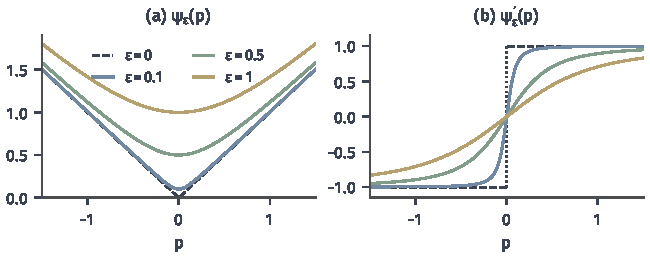
\includegraphics[width=110mm]{figures/03-optimization-evolution-and-signals/01-optimization/matplotlib/c9-smoothed-abs/figure.pdf}
  \caption{一维的平滑导数幅度密度。(a)~$\psi_\varepsilon(p)=\sqrt{p^2+\varepsilon^2}$，$\varepsilon=0.1,0.5,1$，黑色虚线为$\varepsilon=0$时的$|p|$；(b)~导数$p/\sqrt{p^2+\varepsilon^2}$，取值在$(-1,1)$内，在$p=0$处斜率最大，为$1/\varepsilon$。$\varepsilon\to0$时导数趋于在零点跳跃的符号函数（黑色虚线）。}
  \label{fig:opt-fn-smoothed-abs}
\end{figure}

\subsection{Euler--Lagrange方程}
\label{sec:opt-fn-euler-lagrange}

一阶变分~\eqref{eq:opt-fn-first-variation}同时含有$h$和$h'$。若最优条件要求它对许多$h$为零，我们希望把$h'$转移成$h$，得到一个只乘以$h$的积分，再由$h$的任意性推出被积函数为零。分部积分完成转移，代价是出现边界项；先选在边界附近为零的扰动，让边界项消失。

\paragraph{变分基本引理}
用$C_c^\infty(a,b)$表示在$(a,b)$内某个闭子区间外恒为零的光滑函数，称为测试函数。

\begin{lemma}[变分基本引理]
\label{lem:opt-fn-fundamental}
设$w$在$(a,b)$上连续，且$\int_a^bw\varphi\,dx=0$对所有$\varphi\in C_c^\infty(a,b)$成立，则$w\equiv0$。
\end{lemma}

\begin{proof}
若某点$x_0$处$w(x_0)>0$，由连续性存在$\delta>0$使$w>w(x_0)/2$在$(x_0-\delta,x_0+\delta)\subset(a,b)$上成立。取一个在此区间外为零、在区间内为正的光滑凸起函数$\varphi$，则$\int w\varphi>0$，矛盾。$w(x_0)<0$同理。
\end{proof}

$w$只局部可积时，结论改为$w=0$几乎处处，这正是卷二中弱导数唯一性所依据的事实。下面的推导在内部只用测试函数，所以引理适用于约束为固定端点、零扰动迹或其他只限制边界的情形。

\paragraph{一维方程}
设$u^\star$是$J$在某个可行集上的局部最小点，可行集允许所有$u^\star+t\varphi$（$\varphi\in C_c^\infty(a,b)$，$|t|$小），并且~\eqref{eq:opt-fn-first-variation}对这些方向成立。由定理~\ref{thm:opt-fn-first-order-necessary}的论证，
\begin{equation}
 \int_a^b\bigl(F_u\,\varphi+F_{u'}\,\varphi'\bigr)\,dx=0\qquad\text{对所有}\varphi\in C_c^\infty(a,b) .
 \label{eq:opt-fn-weak-el}
\end{equation}
若$x\mapsto F_{u'}(x,u^\star,u^{\star\prime})$连续可微（例如$u^\star\in C^2$且$F$二次连续可微），分部积分，边界项因$\varphi(a)=\varphi(b)=0$消失，得$\int_a^b\bigl(F_u-\frac{d}{dx}F_{u'}\bigr)\varphi\,dx=0$。由引理~\ref{lem:opt-fn-fundamental}，
\begin{equation}
 F_u-\frac{d}{dx}F_{u'}=0\qquad\text{在}(a,b)\text{上} .
 \label{eq:opt-fn-el}
\end{equation}
称为\term{Euler--Lagrange方程}（Euler--Lagrange equation）。没有这样的光滑性时，保留积分形式~\eqref{eq:opt-fn-weak-el}：它恰好说明$F_{u'}$的弱导数存在并等于$F_u$，因为弱导数的定义正是$\int F_{u'}\varphi'=-\int F_u\varphi$对一切测试函数成立。这称为方程的弱形式，只对合法的测试函数断言等式。

\paragraph{多元方程}
在有界Lipschitz区域$\Omega\subset\mathbb R^d$上，用$C_c^\infty(\Omega)$中的测试函数和散度定理代替一维分部积分，相同的论证在足够光滑时给出
\[
 F_u-\operatorname{div}F_{\nabla u}=0\qquad\text{在}\Omega\text{内},
\]
其中对多分量场按分量理解：第$i$个方程为$(F_u)_i-\sum_j\partial_j(F_{\nabla u})_{i,j}=0$。光滑性不足时同样保留弱形式$\int_\Omega(F_u\cdot\varphi+F_{\nabla u}:\nabla\varphi)\,dx=0$。

\paragraph{候选方程与最优性论证}
对固定端点的导数平方能量~\eqref{eq:opt-fn-dirichlet-energy}，$F_u=0$、$F_{u'}=u'$，方程~\eqref{eq:opt-fn-el}化为$u''=0$，满足$u(0)=0,u(1)=1$的解是$u^\star(x)=x$。这一步只得到了候选，最优性另需论证。任取$v\in C$，令$h=v-u^\star\in H_0^1(0,1)$，则
\[
 \begin{aligned}
 J_0(v)&=J_0(u^\star)+\int_0^1h'\,dx+\frac12\int_0^1h'^2\,dx\\
 &=J_0(u^\star)+\bigl[h\bigr]_0^1+\frac12\int_0^1h'^2\,dx=\frac12+\frac12\int_0^1h'^2\,dx .
 \end{aligned}
\]
所以$J_0(v)\ge J_0(u^\star)=1/2$，等号当且仅当$h'=0$几乎处处，结合$h(0)=0$即$h=0$。$u^\star$是唯一的最小点。这里起作用的是平方差展开，也就是$J_0$的凸性，而不是“解出了方程”。

\paragraph{能量与长度}
图~\ref{fig:opt-fn-fixed-endpoint-candidates}比较了几条固定端点的曲线。直线$x$的能量$1/2$与长度$\sqrt2\approx1.414$都最小；弧长的Euler--Lagrange方程$\frac{d}{dx}\bigl(u'/\sqrt{1+u'^2}\bigr)=0$推出$u'$为常数，同样给出直线。最优性仍要单独论证：$\sqrt{1+p^2}$是凸函数，弧长因而是凸泛函，由支撑不等式~\eqref{eq:opt-fn-convex-support}，$\ell(v)\ge\ell(x)+\int_0^1\frac{h'}{\sqrt2}\,dx=\ell(x)$，其中$h=v-x$两端为零。两个目标对其他曲线的评判却不同：$\sqrt x$是$x^2$关于对角线的镜像，长度相同，但它在原点处斜率无界，$\int_0^1u'^2dx=\int_0^1\frac{dx}{4x}=+\infty$，导数平方能量把它排除在$H^1$之外。

\begin{figure}[!htb]
  \centering
  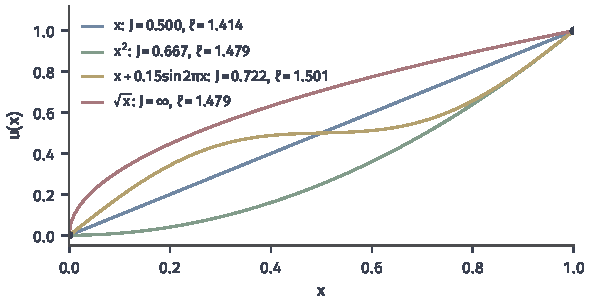
\includegraphics[width=100mm]{figures/03-optimization-evolution-and-signals/01-optimization/matplotlib/c9-fixed-endpoint-candidates/figure.pdf}
  \caption{连接$(0,0)$与$(1,1)$的四条曲线及其导数平方能量$J=\frac12\int_0^1u'^2dx$和弧长$\ell=\int_0^1\sqrt{1+u'^2}\,dx$。直线$x$同时使两者最小（$J=1/2$，$\ell=\sqrt2$）；$x^2$与$\sqrt x$互为镜像，长度同为约$1.479$，后者的能量却是无穷大。}
  \label{fig:opt-fn-fixed-endpoint-candidates}
\end{figure}

\paragraph{非二次能量的内部方程}
对~\eqref{eq:opt-fn-smoothed-tv}，$F_u=0$，$F_{\nabla u}=\nabla u/\sqrt{\|\nabla u\|_2^2+\varepsilon^2}$，内部方程是
\[
 -\operatorname{div}\frac{\nabla u}{\sqrt{\|\nabla u\|_2^2+\varepsilon^2}}=0 .
\]
一维时它说明$u'/\sqrt{u'^2+\varepsilon^2}$为常数，从而$u'$为常数，固定端点下又得到直线。多维时这是一个非线性方程，其解的存在性与正则性不能由这里的推导得到；第~\ref{sec:opt-fn-existence}节将看到，即使存在性论证本身也需要额外的依据。具体方程的解理论由第~\ref{part:dynamical-systems-control-and-decision}部分继续处理。

\subsection{边界条件}
\label{sec:opt-fn-boundary}

上一小节有意让边界项消失。若可行集允许候选在边界上变化，最优条件就会对边界项提出要求；哪些边界扰动合法，由可行集决定。

\paragraph{一维的边界项}
保留分部积分的边界项，在~\eqref{eq:opt-fn-el}所需的光滑性下，
\begin{equation}
 J'(u;h)=\int_a^b\Bigl(F_u-\frac{d}{dx}F_{u'}\Bigr)h\,dx+\Bigl[F_{u'}\,h\Bigr]_a^b .
 \label{eq:opt-fn-boundary-term}
\end{equation}
设最优点$u^\star$只受左端条件$u(a)=\alpha$约束，右端自由。先用测试函数得到内部方程，~\eqref{eq:opt-fn-boundary-term}中的积分对所有合法$h$都消失；再取满足$h(a)=0$、$h(b)=1$的光滑$h$，剩下的边界项给出
\[
 F_{u'}\bigl(b,u^\star(b),u^{\star\prime}(b)\bigr)=0 .
\]
这个条件不是事先规定的，而是由最优性推出的，称为\term{自然边界条件}（natural boundary condition）。直接写进可行集的条件$u(a)=\alpha$则相应地称为\term{本质边界条件}（essential boundary condition）：那里扰动必须满足$h(a)=0$，边界项自动消失，不产生新的方程。

\begin{example}[固定端与自由端]
\label{ex:opt-fn-free-end}
在$[0,1]$上最小化$J(u)=\int_0^1\bigl(\tfrac12u'^2-u\bigr)\,dx$。$F_u=-1$，$F_{u'}=u'$，内部方程为$-u''=1$。两端固定为零时，解是$u=x(1-x)/2$，$J=-1/24$。只固定$u(0)=0$、右端自由时，自然边界条件为$u'(1)=0$，解是$u=x-x^2/2$，$J=-1/6$。两个问题的目标都是凸的，与上一小节相同的平方差展开说明这两个解分别是各自可行集上的唯一最小点。图~\ref{fig:opt-fn-boundary-conditions}中，右端自由的曲线以水平切线到达边界；可行集更大，最小值也更低。
\end{example}

\begin{figure}[!htb]
  \centering
  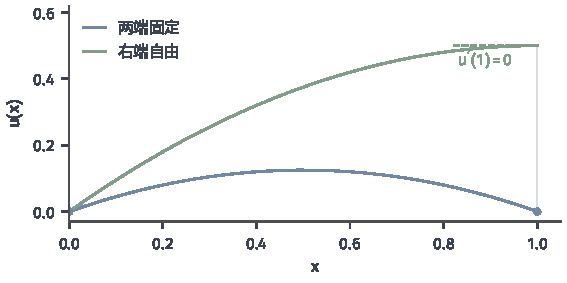
\includegraphics[width=96mm]{figures/03-optimization-evolution-and-signals/01-optimization/matplotlib/c9-boundary-conditions/figure.pdf}
  \caption{同一目标$J(u)=\int_0^1(\frac12u'^2-u)\,dx$在两种边界条件下的最优解。两端固定时（蓝）解为$x(1-x)/2$，$J=-1/24$；右端自由时（绿）解为$x-x^2/2$，在$x=1$处满足自然边界条件$u'(1)=0$，$J=-1/6$。}
  \label{fig:opt-fn-boundary-conditions}
\end{figure}

\paragraph{多元区域的边界}
在$\Omega$上用散度定理，足够光滑时
\[
 J'(u;h)=\int_\Omega\bigl(F_u-\operatorname{div}F_{\nabla u}\bigr)\cdot h\,dx+\int_{\partial\Omega}\bigl(F_{\nabla u}\bm n\bigr)\cdot h\,dS ,
\]
其中$\bm n$是单位外法向量；多分量情形$F_{\nabla u}\bm n$是$m\times d$矩阵乘以$d$维向量，得到$m$维的通量。若边界分为固定部分$\Gamma_D$与自由部分$\Gamma_N$，则$\Gamma_D$上扰动迹为零，$\Gamma_N$上允许任意的边界扰动，于是在$\Gamma_N$上得到$F_{\nabla u}\bm n=0$。若目标还含边界代价$\int_{\Gamma_N}G(x,u)\,dS$，它的一阶变化$\int_{\Gamma_N}G_u\cdot h\,dS$并入边界项，自然条件变为$F_{\nabla u}\bm n+G_u=0$。

\paragraph{梯度场拟合的边界含义}
第~\ref{chap:opt-function-fitting}章用闭子空间投影求得了梯度场拟合问题的解：给定向量场$v\in L^2(\Omega;\mathbb R^d)$，最小化$\frac12\int_\Omega\|\nabla u-v\|_2^2dx$，并由投影余项的正交性得到$\int_\Omega(\nabla u-v)\cdot\nabla h\,dx=0$。这正是密度$F=\frac12\|\nabla u-v\|_2^2$的一阶条件，$F_{\nabla u}=\nabla u-v$。足够光滑时，内部给出$\operatorname{div}(\nabla u-v)=0$；若边界自由，自然边界条件是
\[
 (\nabla u-v)\cdot\bm n=0\qquad\text{在}\partial\Omega\text{上} .
\]
它不能无条件改写成$\partial_{\bm n}u=0$：只有当$v\cdot\bm n=0$时二者才一致。点态的通量条件需要额外的正则性，条件不足时只保留弱形式。拟合解的存在与唯一已在上一章证明，这里只补充边界条件的含义。

\paragraph{纯导数能量的自由边界}
对~\eqref{eq:opt-fn-smoothed-tv}在自由边界下作同样的推导，自然边界条件是$\nabla u\cdot\bm n/\sqrt{\|\nabla u\|_2^2+\varepsilon^2}=0$，即$\partial_{\bm n}u=0$。由于$\psi_\varepsilon(\bm p)\ge\varepsilon$，等号当且仅当$\bm p=0$，所以$J_\varepsilon(u)\ge\varepsilon|\Omega|$，等号恰在$\nabla u=0$时成立：在连通区域上任何常函数都是最小点。纯导数能量只奖励平坦，本身不含保持某个给定信号的要求；要让结果贴近数据，目标中必须另有观测项。
